\newpage
\section{Metodologia Experimental}

\subsection{Materiais}
O material utilizado foi:

\begin{itemize}
	\item Protótipo do conversor Buck disponível no laboratório;
	\item CI 3524;
	\item AmpOp LM324;
	\item 2 potenciômetros de 10 $k \, \Omega$;
    \item 6 resistores de 1 $k \, \Omega$;
    \item 1 capacitor de 1 $nF$;
    \item 1 termistor de 10 $k \, \Omega$;
	\item Osciloscópio;
	\item Multímetro;
	\item Resistor variável de potência (50 $\Omega$).
\end{itemize}

Para execução do experimento, faz-se necessário executar os seguintes passos:

\begin{enumerate}
    \item montar o protótipo Buck (figura \ref{fig:buck}) com tensão de entrada de 30V.
	\item montar o circuito do controlador conforme a figura \ref{fig:sch}, alimentando o CI com 12V;
	\item ajustar o circuito para responder as perguntas da seção \ref{perguntas}.
\end{enumerate}

\begin{figure}[H]
    \centering
    \caption{Montagem do conversor Buck.}
    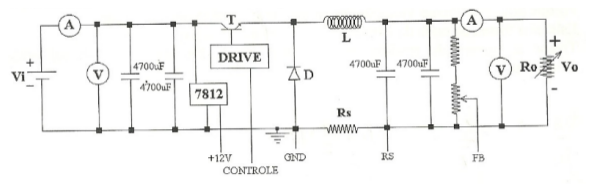
\includegraphics[scale=0.5]{buck}
    \label{fig:buck}
\end{figure}

\begin{figure}[H]
	\centering
	\caption{Controlador com CI SG3524.}
	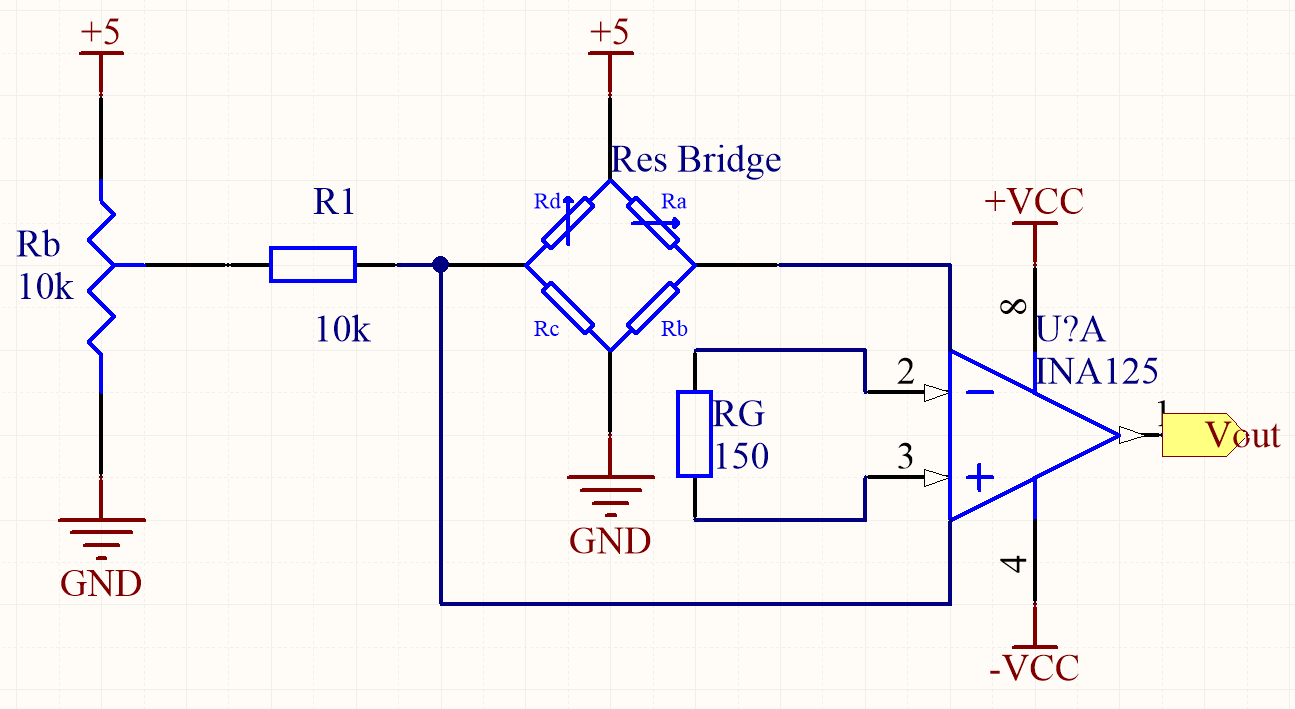
\includegraphics[scale=0.6]{sch}
	\label{fig:sch}
\end{figure}



\subsection{Questões}
\label{perguntas}

\begin{enumerate}
    \item Para ajustar a frequência dos pulsos de controle, utilizar um capacitor de 1 nF e potenciômetro de 10 $k \, \omega$; Variando o potenciômetro, ajuste a frequência de saída para 100 kHz com $K_c = 0.5$. Qual a frequência de saída se o $K_c$ for alterado para 1?
    
    \item Variando o potenciômetro, ajuste a frequência de saída para 50 kHz (ou um valor próximo a este) com $K_c = 0.5$. Qual é a frequência de saída se o $K_c$ for alterado para 1?
    
    \item Simular um aumento de temperatura utilizando um ferro de solda e o termistor NTC para cortar os pulsos de comando através do pino \textit{shutdown} do 3524;
    
    \item Para o controlador com $K_c = 0.5$ e frequência 100 kHz, qual a tensão de saída do conversor buck tendo como carga 25 $\omega$ / 1kW (ajustar o reostato para este valor)?
    
    \item Para o controlador com $K_c = 1$ e frequência 100 kHz, qual a tensão de saída do conversor buck tendo como carga 25 $\omega$ / 1kW (ajustar o reostato para este valor)?
    
    \item Quais os conversores que devem utilizar o $K_c = 0.5$? Cite três conversores.
    
    \item Quais os conversores que devem utilizar o $K_c = 1$? Cite três conversores.
    
\end{enumerate}